% !TEX root = ../main.tex

\chapter{绪论}


\section{引言}

编译器作为关键系统软件之一,其正确性对于计算机系统的安全运行有重要意义。
这是由于编译器可能在转换程序的过程中引入错误,导致目标程序的行为和源程序不一致,
进而使得在源程序端花费大量精力的测试和验证工作在目标程序层级失效。
虽然对于编译器一般会进行密集的测试,错误编译是小概率事件,但是这种偶发性的
由编译器引入的问题,对于安全关键系统而言是需要考虑的。
工业界长期以来对保障编译器正确性这个问题非常重视。例如,按照航空领域的RTCA DO178B/C标准~\cite{brosgol2010178c},
需要按照和机载软件一样的严格要求对待编译器。
对于庞大的编译器,通过测试找到它的错误其实是比较困难的。
编译器随机测试工具Csmith~\cite{csmith2011}已经发现了四百多个编译器错误,可见编译器中隐藏的风险数量之大。

编译器的形式化验证已被证实可以有效保证编译器的正确性,它从数学层面上确保了编译过程的正确性。
一个著名的例子是经过验证的C编译器CompCert~\cite{leroy2009formally},
它将C语言的一个有代表性的重要子集编译到了支持多种处理器架构的汇编代码(包括PowerPC、ARM、X86和RISC-V)。
其编译过程的正确性(即目标汇编程序保存了源C程序的语义)经过了形式化验证,并在Coq定理证明器中实现。

延续传递风格(Continuation-Passing Style, CPS)是一种函数式程序的中间语言(Intermediate Representation, IR),
它明确了函数式程序的控制流,从而为程序基于控制流的分析和优化提供了便利。
延续传递风格的中间语言在函数式程序的编译器中被
广泛采用\cite{belanger-cpp2013,dargaye2009verification,zoe-oopsla2021,zoe-icfp2021,wang-esop2016}。
然而,这也意味着经验证的函数式编译器不能直接得到主流编译器基础设施(例如LLVM和GCC)的支持。
这些主流编译器基础设施采用静态单赋值(Static Single Assignment, SSA)形式的中间语言。 
SSA中间语言在工业编译器中大大流行,因为它可以通过强制让每个变量只能被赋值一次来实现
便捷而准确的数据流分析(Data-Flow Analysis, DFA),进而实现各种基于数据流分析的激进优化。
许多流行的命令式编程语言(例如Rust~\cite{balasubramanian2017system}和Swift~\cite{zhang2012swift})
使用这些编译器基础设施作为其后端,生成性能优越的代码~\cite{lattner2006introduction}。
一些工业级的函数式编译器也开始采用SSA形式的中间语言。例如,SML-New Jersey的
新版本已经将其后端转向了LLVM~\cite{farvardin2020new}。

在本文中,我们研究了如何构建基于SSA中间语言的经验证的函数式语言编译器。
具体而言,我们设计并验证了从CPS到SSA的转换算法,以便在经验证的编译器领域中将
传统基于CPS的函数式编译器与基于SSA中间语言上工作的主流编译器后端连接起来。
尽管研究人员已经探讨了CPS和SSA程序结构之间的对应关系~\cite{appel1998ssa,ssabook},
和相互转换~\cite{farvardin2020new,kelsey1995correspondence},
但如何对转换算法进行形式化验证仍然是待解决的问题。

本文的主要贡献总结如下:

\begin{itemize}
    \item
    我们的主要贡献是设计和验证了从CPS到SSA的转换算法。该转换过程的源语言是代表性的
    函数式语言PCF\cite{plotkin1977lcf},我们首先需要将其转换为CPS形式。
    转换算法的SSA目标语言是LLVM IR的一种简化版本,保留了LLVM IR的基本结构。
    该转换是基于CPS和SSA结构上的对应关系设计的~\cite{appel1998ssa,kelsey1995correspondence}。
    我们为PCF和SSA语言定义了小步操作语义,使用基于模拟的方法证明目标程序实现了
    源程序的语义保存。据我们所知,这是第一个经过验证的从CPS函数式程序到SSA的转换。
    
    \item 
    我们还利用该经验证的编译链构建了PCF语言的编译器原型。它是部分经过形式化验证的,
    为未来构建更复杂更完整的经验证函数式语言编译器打下基础。
    具体而言,我们首先实现并验证了直接风格PCF语言的CPS转换,并将它连接到经验证的CPS到SSA的编译过程。
    然后,我们通过Vellvm提供的抽象语法(Vellvm是一个经过验证的LLVM基础设施~\cite{zakowski2021modular}),
    将SSA中间语言转换为LLVM IR。
    
\end{itemize}

在本章接下来的内容中,我们首先在\ref{sec:background}节介绍必要的相关背景知识,
并在\ref{sec:related}节讨论了领域内与本课题相关的工作。
在第\ref{ch:overview}章中,我们简要介绍了该部分经验证的PCF编译器原型。
我们在第\ref{ch:trans}章中讨论了CPS转换和CPS到SSA的转换算法设计,
并在第\ref{ch:verify}章中对该编译链进行形式化验证。
本文工作在Coq中的实现和评估将在第\ref{ch:implement}章中介绍。
最后,我们在第\ref{ch:summary}章中对本文内容进行总结。

\section{相关背景} \label{sec:background}

在本节中,我们将对该课题的相关背景进行介绍。
本文工作涉及函数式编程、编译器常用中间语言形式以及编译器形式化验证方法等方向。
首先,我们会介绍函数式编程的概念及其特性。
然后,我们将说明CPS形式是如何帮助函数式程序显式地表示控制流的,
并介绍了静态单赋值中间语言的相关特性以及CPS和SSA结构之间的对应关系。
接下来,我们介绍了在经验证的编译器CompCert中提出的基于模拟技术进行编译器验证的框架~\cite{leroy2009formally}。

\subsection{函数式编程}

函数式编程(Functional Programming)是一种通过应用和组合函数来构建程序的编程范式,
以$\lambda$演算($\lambda$-Calculus)作为其数学基础~\cite{church1985calculi}。
传统命令式编程中,计算通过执行程序语句序更新程序状态来实现。
相比之下,函数式编程中程序由包含函数定义和应用的表达式构成,而计算通过对表达式求值来实现。
函数式程序的一大特点是函数可以作为参数传递,或者被其他函数返回,形成所谓的高阶函数~\cite{sussman1998scheme}。
此外,纯粹函数式程序的执行不会引起改变程序状态的副作用。
这些特点使得函数式程序设计语言编写的程序更加简洁、安全和易于验证~\cite{hudak1989conception},
因此在并发编程、系统内存编程等方面获得了成功应用。

在学术界和工业界中,函数式编程的应用日趋广泛。
除了Haskell~\cite{o2008real}等纯函数式语言,OCaml、Erlang、Scala~\cite{cesarini2009erlang, odersky2014unifying}
等语言都对函数式编程有内生的支持,且诸多命令式编程语言如C++和Rust也在积极的引入函数式编程机制。
本文研究的函数式编程语言是学术界有广泛影响力的PCF(Programming Computable Functions)。
由于PCF可以看作是工业用函数式编程语言的核心,本文的研究结果可被推广至其他函数式语言。
关于PCF语言的更多特性将在第\ref{sec:cps}节中详述。

\subsection{延续传递风格与静态单赋值} \label{sec:bg_cpsssa}

函数式程序的形式有很多种,如直接风格(Direct Style)和延续传递风格(CPS)。
图~\ref{cpsdirect}展示了同样含义的函数式程序在这两种不同表示风格下的例子。
CPS的关键特性在于通过延续明确地表示程序的控制流。
CPS中的延续(Continuation)指的是当前执行节点后所有剩余计算的函数,
该函数需要把当前计算得到的结果作为其输入。
具体来说,CPS函数需要将延续作为额外的参数传入,
当运行该函数得到计算结果后,程序通过调用该延续来传递这个值,也就是``返回''该结果。
以图~\ref{fig:cps2}为例,函数$h$在CPS中的延续参数为$k$,在得到最终结果$z$之后,
程序调用$(k\; z)$以返回$z$,并执行$k$所代表的剩余计算。
当调用CPS函数时,调用者需要提供一个延续函数来表示剩余计算,且在CPS中所有中间结果、控制流中的控制点都需要被明确命名。
这些特点导致用户直接用CPS形式编写代码较为困难,但是由于明确表示的控制流利于程序分析和优化,
CPS是函数式语言编译器中常见的中间表示形式。

\begin{figure}
    % \vspace{-0.3cm}
    \centering
    \begin{subfigure}[b]{0.3\textwidth}
        \flushright
    % \small
     \begin{equation}
        \nonumber
        \begin{aligned}
        &  \mathbf{function}\; h(x,y) = \\
        & \quad (x*x)\; +\; (y*y) \\
        \end{aligned}
    \end{equation}
    \caption{Direct Style}
        \label{fig:ori2}
    \end{subfigure}
 %   \hfill
    \begin{subfigure}[b]{0.6\textwidth}
        \flushleft
        % \small
        \begin{equation}
            \nonumber
            \begin{aligned}
            & \mathbf{function}\; h(x,y,k)= \mathbf{let}\; x_1=x*x\; \mathbf{in} \\
            &  \quad   \mathbf{let}\; y_1=y*y\; \mathbf{in}\; (\mathbf{let}\; z=x_1+y_1\; \mathbf{in}\; (k\; z)) \\
            \end{aligned}
        \end{equation}
        \caption{CPS}
        \label{fig:cps2}
    \end{subfigure}
    \caption{直接风格和CPS形式的示例函数式程序}\label{cpsdirect}
  \end{figure}

Plotkin~\cite{plotkin1977lcf}、Danvy和Nielsen\cite{danvy2007one}等人研究了将直接风格的函数式程序转换为CPS程序的方法。
其中Plotkin的方法需要后续进行管理性缩减(Administrative Reduction),以去除冗余的$\lambda$结构。
Felleisen等人提出了另一种方法非组合式的方法,其基于$\lambda$-演算的语义。
Danvy和Nielsen将这两种方法联系起来,可以只通过一步转换完成,不需要在后续过程中进行管理性缩减。

静态单赋值(SSA)是命令式语言编译器中一种广泛使用的中间语言类型。
在SSA中,每个变量只能在一处被赋值,且被使用之前必须已经被赋值。
这种性质很接近函数式语言中的名字绑定(Name Binding)~\cite{ssabook}。
变量被划分为不同的版本,新版本的变量往往使用原名加下标来表示,以使每个定义得到自己的版本。
$\phi$节点($\phi$-nodes)作为特殊的程序语句被插入到基本代码块的开头,
从而按照前驱基本块的名字生成新变量的赋值语句。
这样一来,变量的使用定义链(Use-def Chains)更加清晰,从而使许多编译器优化算法
在SSA中间语言上能够更好地实现,例如常量传播、无用代码消除、寄存器分配等~\cite{ssabook,kelsey1995correspondence}。
作为示例,图~\ref{ssacfg}展示了一个SSA程序的控制流图(Control-Flow Graph)。
其中,基本代码块$b_2$的前驱基本块可以是$b_1$或$b_2$本身。
不同的前驱基本块对变量$y$有不同的赋值,在$b_1$和$b_2$中变量$y$被赋予了不同版本的名称。
基本块$b_2$开头的$\phi$节点将$y_1$和$y_3$作为参数,根据执行时控制流的实际前驱基本块来
选择正确的版本赋值给新的变量$y_2$。

LLVM IR就是一种基于SSA的中间代码。它作为一种高层次的汇编语言,提供了编译系统的中间层,
使得不同语言可以相互连接起来,复用其后端优化~\cite{lattner2006introduction}。
除了LLVM,还有很多编译器是基于SSA的,例如GCC编译器的中间语言GIMPLE~\cite{callanan2007extending}、
面向微软.NET平台的即时编译中间语言CIL(Common Intermediate Language)~\cite{thai2003net}等。

\begin{figure}[htbp]
    \centering
    % \documentclass{article}
% \usepackage{tikz}
% \usetikzlibrary{chains,shadows.blur}

% \begin{document}
\begin{tikzpicture}[auto,
%   node distance = 12mm,
%   start chain = going right,
  box/.style = {draw,rounded corners,blur shadow,fill=white,
        align=center}]
 \small
 \node[box] (b1) at(0,0)    {$v_1 \leftarrow 1$\\ 
                    $z_1 \leftarrow 8$ \\ 
                    $y_1 \leftarrow 4$};      
 \node[box] (b2) at(3,0)    {$y_2 \leftarrow \phi(y_1,y_3)$\\
                    $x_1 \leftarrow 5 + y_2$ \\
                    $y_3 \leftarrow x_1 * z_1$ \\
                    $x_2 \leftarrow x_1 - 1$ \\
                    $\mathbf{if}\; x_2 = 0$};      
 \node[box] (b3) at(6.5,0)    {$w_1 \leftarrow v_1 +y_3$\\ 
                    $\mathbf{return}\; w_1$};  
 \node at(4.0,1.5) {false};
 \node at(4.8,0.3) {true};

 \coordinate (b1n) at ([yshift=-31] b1);
 \coordinate (b2n) at ([yshift=-43] b2);
 \coordinate (b3n) at ([yshift=-25] b3);

 \node at (b1n)  {$b_1$};
 \node at (b2n)  {$b_2$};
 \node at (b3n)  {$b_3$};
 
 \begin{scope}[rounded corners,-latex]
  \path (b2.60) edge[bend right=50] (b2.120)
        (b1) edge (b2) (b2) edge (b3) ;
%   \draw (b3.230) -- ++(0,-0.3) -| ([xshift=-5mm]b2.west) |-
%   ([yshift=3mm]b2.130) -- (b2.130);
 \end{scope}
\end{tikzpicture}
% \end{document}      
    \caption{SSA程序的控制流图示例}\label{ssacfg}
\end{figure}

Appel等人~\cite{appel1998ssa}发现SSA也是一种函数式语言:$\lambda$演算和SSA虽然有不同的形式,
但它们所做的工作其实是相同的。L. Beringer~\cite{ssabook}给出了SSA的函数式表示,
将SSA中的相关术语与函数式编程中的概念联系起来。
例如,函数式语言中的$let$绑定对应着SSA中的赋值、绑定变量的词法作用域对应着SSA中的可支配区域。
$let$绑定与变量定义点之间的对应关系还延续到了程序结构的其他方面。
与命令式语言中的返回地址或函数指针相似,延续指定了当前代码片段求值完成后程序下一步该如何执行。
SSA中的控制流图对应着函数式编程中的函数,虽然顶层延续的参数在控制流图中并不是明确可见的,
但它对应一个命令式调用中用来保存返回地址的地方。
Kelsey~\cite{kelsey1995correspondence}通过将CPS中的$\lambda$进行标注来区分完整过程、跳转、延续,
进而将被这种标注的CPS程序转换为一种SSA程序。然而,Kelsey工作中的CPS和SSA语言与本文中所使用的差距较大。
Kelsey的CPS语言将二元表达式的参数和条件语句中的条件视为表达式,使其更类似于带有延续元素的标准函数式程序。
例如,在Kelsey的工作中,表达式$k; ((x+y)+z)$是允许的,但在我们的工作中,
它必须转换为$\mathbf{letop}; x_0 = x+y; \mathbf{in}; (\mathbf{letop}; x_1 = x_0+z; \mathbf{in}; k; x_1)$。
此外,Kelsey的转换算法选择先合并CPS过程,然后再将其作为整体进行转换。
因此,SSA程序的顶层单元是一整个过程,没有函数调用,这与本文中使用的基于LLVM IR的SSA语言不同。

\subsection{编译器形式化验证} \label{sec:compcertbackend}

我们使用CompCert~\cite{leroy2009formally}基于模拟(Simulation)技术的形式化验证框架来证明转换过程的正确性。
经过形式化验证的C语言子集编译器CompCert是由INRIA的Xavier Leroy领导开发的,在Coq定理证明工具中实现。

CompCert已被应用于诸如核电站控制软件和飞行控制系统的开发。
清华大学王生原、尚书等人设计并实现了基于CompCert的L2C编译器~\cite{shang2017key},被用于安全关键的工业领域。
L2C的源语言是被广泛用于安全关键的工业领域(高铁、核电站等)的 Lustre,
这些类型的应用对开发工具本身的安全性要求很高。它的目标语言是ComperCert中使用的C子集Clight。
南京大学冯新宇等人针对并发程序进行了单独编译验证~\cite{jiang2019towards}。他们提出了独立于语言的验证框架,
将顺序程序与无竞赛并发程序编译器验证工作联系起来,从而使针对顺序程序的编译器验证工作可以被重用。
使用这种框架,他们建立了CASCompCert。它扩展了ComperCert,可以对无竞赛Clight并发程序的单独编译进行验证,
且允许将并发Clight模块与包含良性竞赛的同步原语的x86-TSO实现进行连接。

CompCert提供了一套基于模拟技术验证编译过程正确性的理论和框架。该框架将编译过程的正确性定义为
语义保存性质(Semantic Preservation Property),即目标程序的行为应该与源程序的行为一致。
我们将程序的行为(Behaviors)描述为由小步操作语义(Small-Step Operational Semantics)生成的轨迹(Trace),
以便直接推导出编译器的正确性证明。根据CompCert中对语义保存性质的讨论,
通过为安全的源程序建立后向模拟(Backward Simulaion),可以证明语义保存性质。

接下来,我们会介绍一些概念来说明什么是安全程序的后向模拟。
可以通过程序语言的语义将可观察行为(Observable Behaviors)与程序关联起来。
程序的可观察行为可以分为终止(Termination)、发散(Divergence)和出错(Going wrong)。
如果用$P_1$表示源程序,$B$表示可观察行为,那么$P_1 \Downarrow B$表示执行程序$P_1$获得的可观察行为为$B$。
同样的表示方法也可以应用于目标程序。在CompCert框架中,仅对不会出错的安全的源程序提供正确性保证。
如果我们将编译过程表示为$\mathcal{T}$函数,则经过转换得到的目标程序可以表示为$\mathcal{T}(P_1)$。
编译安全程序的正确性可以描述为目标程序的行为是可接受的源程序行为。
那么,安全源程序的后向模拟可以表示为:如果$P_1$是一个安全程序,
则对于所有的可观察行为$B$,$\mathcal{T}(P_1) \Downarrow B \Longrightarrow P_1 \Downarrow B$。

然而,直接证明后向模拟是比较困难的。可以先建立从安全源程序到目标程序的前向模拟(Forward Simulation),
再根据目标程序的确定性和前向模拟来推导出后向模拟。
安全源程序的前向模拟可以表示为:如果$P_1$是一个安全程序,则对于所有的$B$,
$P_1 \Downarrow B \Longrightarrow \mathcal{T}(P_1) \Downarrow B$。
由于目标程序是确定性的(Deterministic),它只与一种行为相关联。
因此,目标程序不会具有$P_1$没有的额外行为。在这种情况下,可以从前向模拟中导出安全程序的后向模拟。

为了证明源语言$L_1$转换为目标语言$L_2$的编译过程满足前向模拟性质,
关键在于建立程序状态$S_1$和$S_2$之间的不变式(Invariant)$S_1\sim S_2$,
并证明它在源程序和目标程序的执行过程中始终成立。
按照CompCert的方法,我们首先需要为$L_1$和$L_2$定义操作语义。
对于任何源程序$P_1$和目标程序$P_2$,我们需要证明$P_1$和$P_2$的初始状态满足不变量$\sim$。
然后,我们需要证明它们的内部执行步骤始终可以通过$\sim$相关联。
也就是说,假设$S_1\sim S_2$,源程序的状态在一步执行后从$S_1$转换到$S'_1$,
那么目标程序状态从$S_2$转换到某个$S'_2$,需要保证在转换后$S'_1\sim S'_2$成立。
根据从$S_2$到$S'_2$的转换步骤数量,可以将模拟图(Simulation Diagram)分为以下几种:

\begin{figure}[ht]
    % \vspace{-10pt}
    \centering
    \begin{subfigure}[b]{0.26\textwidth}
        % \flushleft
        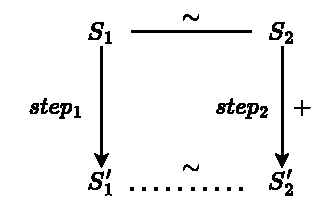
\includegraphics[width=1\linewidth]{figures/plusstep.pdf}
        \caption{多步模拟}
        \label{fig:plus}
    \end{subfigure}
    \begin{subfigure}[b]{0.52\textwidth}
        % \flushright
        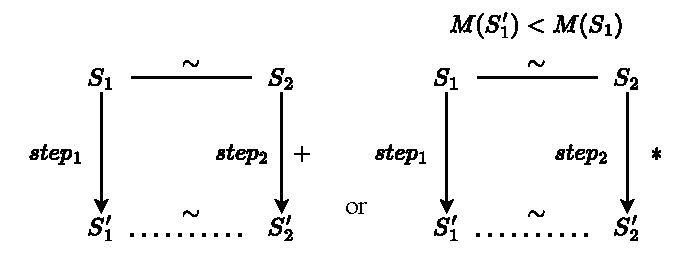
\includegraphics[width=1\linewidth]{figures/starstep2.pdf}
        \caption{星形模拟}
        \label{fig:star}
    \end{subfigure}
    \caption{不同类型的模拟图}\label{simustep}
\end{figure}

\begin{itemize}
    \item 一步模拟(Lock-Step Simulation)表示$S_2$经过一步转换到达$S'_2$状态。
        然而,对于大多数转换算法来说,一步模拟的前提要求太严格了,我们需要对其进行放宽。
    \item 多步模拟(Plus Simulation)表示$S_2$经过一步或多步转换到达$S'_2$(如图~\ref{fig:plus})。
        有时,从$S_1$到$S'_1$的转换对于状态$S_2$没有任何影响,比如删除冗余代码。
        因此,在某些情况下,多步模拟的条件也需要放松。
    \item 星形模拟(Star Simulation)表示$S_2$经过零步或一步或多步转换到达$S'_2$状态(如图~\ref{fig:star})。
        在这种条件下,可能会出现一种违反语义保存性质的情况:源程序发散,而目标程序保持在$S_2$状态,
        它们之间的状态仍然始终满足$\sim$不变式。为了防止出现这种``无限驻留''问题,我们需要
        为源程序的状态定义一个度量函数$M$,它随着源程序的执行过程严格减小。
        增添了度量函数$M$相关的限制,我们就能通过模拟保存源程序的发散行为了。
\end{itemize}

正如我们将在第~\ref{ch:verify}章中讨论的那样,CPS转换的前向模拟满足多步模拟性质,
而对于CPS到SSA的转换,我们需要使用星形模拟。根据上述模拟图性质以及
源程序和目标程序初始状态的对应关系,我们可以推导出安全程序的前向模拟。
结合目标语言的确定性,即可推导出安全程序的后向模拟。

由于语义保存性质是可传递的(Transitively Composable),
我们可以先分别证明各个编译过程的语义保存性质,然后将结果组合起来推导出整个编译过程的正确性。
例如,如果编译过程$\mathcal{T}$被分解为两个转换阶段$\mathcal{T}_1$和$\mathcal{T}_2$,
$\mathcal{T}$可以被视为它们的组合。对于一个安全的程序$P$,如果没有发生编译时错误(Compiler-Time Error),
$\mathcal{T}(P) = \mathcal{T}_2(\mathcal{T}_1(P))$。
如果我们可以验证$\mathcal{T}_1$和$\mathcal{T}_2$的正确性,那么$\mathcal{T}$也得到了验证。

\section{相关工作} \label{sec:related}

在编译器验证领域,许多工作是围绕CompCert编译器展开的,包括很多函数式语言编译器的验证工作。
例如,经验证的函数式编译器CertiCoq将Gallina(Coq语言)编译到了CompCert中使用的的Clight~\cite{belanger2019certified}。
miniML经验证的编译器也使用了CompCert框架,将其编译到了CompCert中的中间语言Cminor~\cite{dargaye2009verification}。
基于SSA的中间语言(例如LLVM IR)模块化、可移植和优化潜能大等特性引起了函数式编译器开发者的关注。
近年来,一些原本不使用SSA后端的函数式编译器已经开始转向SSA后端以获得更好的性能~\cite{farvardin2020new}。
我们的工作基于这些观察建立,是朝着构建利用SSA中间语言优势的经验证的函数式编译器迈出的第一步。

\subsection{Gallina经验证的编译器CertiCoq}

CertiCoq将Gallina编译到了C语言的子集Clight,以便与CompCert链接起来并最终编译到汇编语言,
从而获得一个完整的经过验证的编译链~\cite{belanger2019certified,zoe-oopsla2021,zoe-icfp2021}。
从CPS到Clight的编译过程及其形式化证明在Coq中实现,不过其使用的是大步操作语义而不是小步操作语义。
该编译器的目标语言不是基于SSA的,因此不能直接连接到LLVM框架,也不能利用基于SSA中间语言的优化。

\subsection{miniML经验证的编译器前端MLCompCert}

MLCompCert是Zaynah Dargaye等人设计的一个经验证的编译器前端~\cite{dargaye2009verification}。
它的源语言是ML纯函数式语言的部分,即miniML,包括了$\lambda$演算、$let$绑定、模式匹配等。
它的目标语言是CompCert编译器后端的中间语言Cminor,即一种类似于C语言的底层语言。
该编译器实现了一些经典的函数式程序编译优化,例如反柯里化(uncurrying)和统一数据结构表示等。
设计者们在Coq中对该函数式程序编译器前端进行了实现和验证。

\subsection{SML-New Jersey基于LLVM编译器后端的版本}

SML-New Jersey编译器(SML/NJ)是Standard ML的著名编译器。在最近发布的新版本中,它更改了后端,
将CPS中间语言编译到了LLVM IR~\cite{farvardin2020new}。CPS程序首先被转换为控制流图(Control-Flow Graph, CFG)中间语言,
然后再转换为LLVM IR。这是因为将CPS中间语言连接到基于SSA的编译器基础设施能够利用这些编译器提供的丰富后端优化。
但这项工作不是经过形式化验证的。
我们的工作受到了这一趋势的启发,并进一步尝试对这种连接进行形式化验证。

\subsection{CompCert支持SSA的扩展CompCertSSA}

经验证的编译器也开始试着支持基于SSA中间语言的后端了。
CompCertSSA是CompCert的一个扩展,具有一个基于SSA的中间端~\cite{compcertssa}。
它将SSA作为一种可选的优化中间语言,允许在RTL(Register Transfer Language)三地址代码和SSA中间语言之间进行转换。
虽然这使得CompCert能够实现一些基于SSA的优化~\cite{compcertssa-op,blazy-cpp2023},
但是CompCertSSA提供的优化仍然比较有限,不能与LLVM的后端优化相媲美。
不过,它提供了一个从C语言开始的经过完整验证的编译链,是开发针对SSA的经验证的函数式编译器的有力工具。

\subsection{经验证的LLVM IR: Vellvm}

Vellvm在定理证明工具Coq中定义了LLVM中间语言的抽象语法树(Abstract Syntax Tree, AST),并为LLVM IR提供了形式化语义。
早期版本的Vellvm提供了LLVM IR的操作语义~\cite{zhao2012formalizing},
而在较新版本中已迁移到了基于交互树(Interactive Tree, ITree)的语义~\cite{zakowski2021modular}。
在本文第\ref{ch:overview}章所介绍的编译链中,SSA程序首先被编译到了Vellvm AST,然后生成了最终的LLVM IR程序。
